\section{Manual de Usuario}
\subsection{Introducción}
En esta sección se detallan los pasos a seguir para el uso adecuado del software Detector de Pivotes de Riego y Silo bolsas en Imágenes Satelitales para aplicaciones agrícolas.

\subsection{Pre-requisitos}
Contar con Docker instalado en la computadora.

En el caso de no optar por el uso de Docker, se puede correr localmente de contar con los siguientes requerimientos:
\begin{itemize}
    \item Distribución Linux: Debian o Ubuntu preferentemente (o sus derivados).
    \item Python 3.7 o superior.
    \item Virtualenv.
\end{itemize}

\subsection{Instalación}
\begin{enumerate}
    \item Descargar o clonar el repositorio desde Github: \url{https://github.com/gianfrancob/detector_pivotes_silobolsas}
    \item Inicializar el contenedor Docker corriendo: 
    \begin{itemize}
            \item \textit{docker build -t detector\_pivotes\_silobolsas }
            \item \textit{docker run -p 5000:5000 --name test -it detector\_pivotes\_silobolsas}
    \end{itemize}
    
    \item En el caso de no optar por el uso de Docker, se puede correr localmente de la siguiente manera:
    \begin{itemize}
        \item Crear entorno virtual usando virtualenv: \textit{virtualenv venv}
        \item Activar el entorno: \textit{source ./venv/bin/activate}
        \item Instalar las dependencias en el entorno: \textit{pip install -r ./requirements.txt}
    \end{itemize}
    \item Iniciar el servicio backend: \textit{python ./utils/flask\_rest\_api/restapi\_pivot\_silobolsa.py --port 5000}
    \item Ingresar a la página abriendo en el navegador el siguiente fichero HTML: \textit{./utils/boostrap\_frontend/index.html}
\end{enumerate}

xt

\subsection{Ingresar a la página}
Para ejecución local, la dirección URL donde se encuentra la aplicación es: 
\textit{DIRECTORIO RAIZ/utils/boostrap\_frontend/index.html}

Para ejecución web, dependerá particularmente del tipo de despliegue implementado.

\subsection{Cargar una imagen}

\begin{figure}[b!]
    \centering
    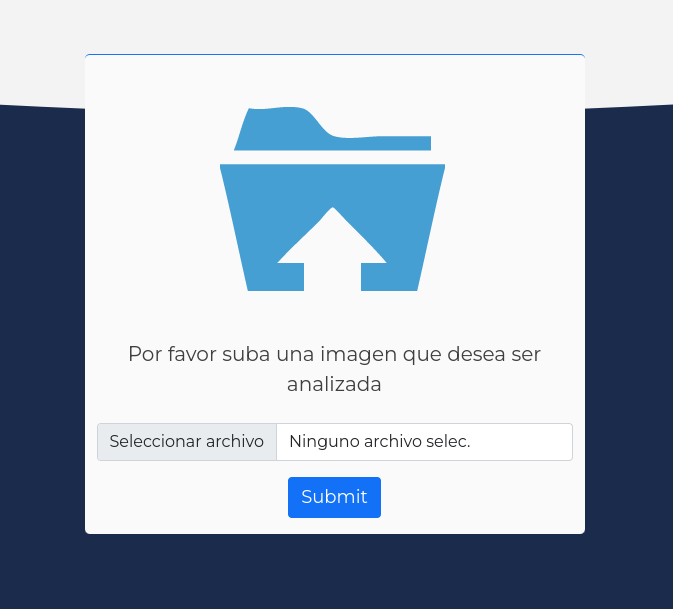
\includegraphics[width=0.8\textwidth]{img/FE - upload file.png}
    \caption{Subir una imagen para analizar}
    \label{fig:subir imagen}
\end{figure}

Una vez en la página principal, dirigirse al botón "Seleccionar archivo" que se encuentra en la mitad de la misma y hacer clic en él para seleccionar una imagen o desde la computadora del usuario, los formatos soportados son .jpg, .png .

\subsubsection{Error en el formato de la imagen}

Si el formato de la imagen cargada esta dañado o es invalido, se mostrara el siguiente mensaje, como se muestra en la figura \ref{fig:error}:

\begin{figure}[h!]
    \centering
    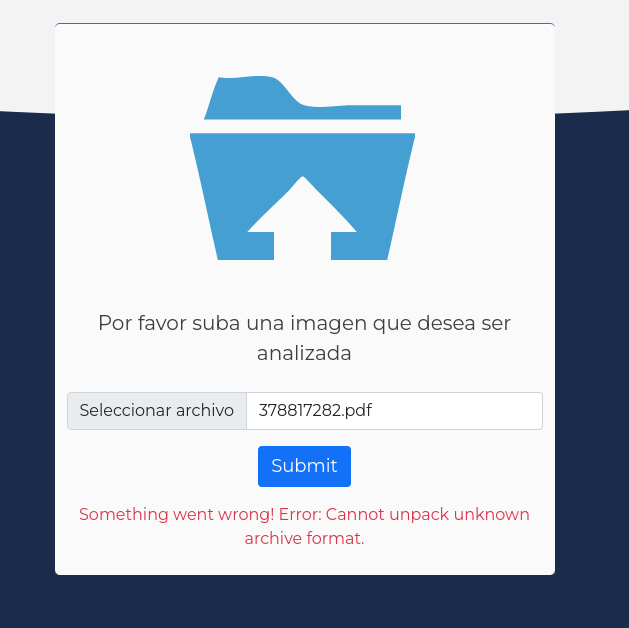
\includegraphics[width=0.6\textwidth]{img/FE - upload error.png} 
    \caption{Error al subir una archivo de formato invalido}
    \label{fig:error}
\end{figure}

\subsection{Cargar varias imágenes} 

Para la opción del análisis de un conjunto de imágenes, previamente se debe crear un archivo de compresión con todas las imágenes en alguno de los siguientes formatos: RPM (.rpm), RAR (.rar), RZIP (.rz), TAR (.tar), XZ (.xz), ZIP (.zip, .jar), GZIP (.gz), 7z (.7z).

Luego, hacer clic en el botón "Seleccionar archivo" para subir el archivo con todas las imágenes a ser analizadas.

\textbf{Nota}: No debe salir ningún mensaje de error para continuar con el análisis,  ver imagen \ref{fig:error}

\subsection{Inicio de la detección} 

Una vez cargada la imagen o las imágenes en formatos validos, hacer clic en el botón \textbf{"Submit"}, para dar inicio a la detección. 

\begin{figure}[h!]
    \centering
    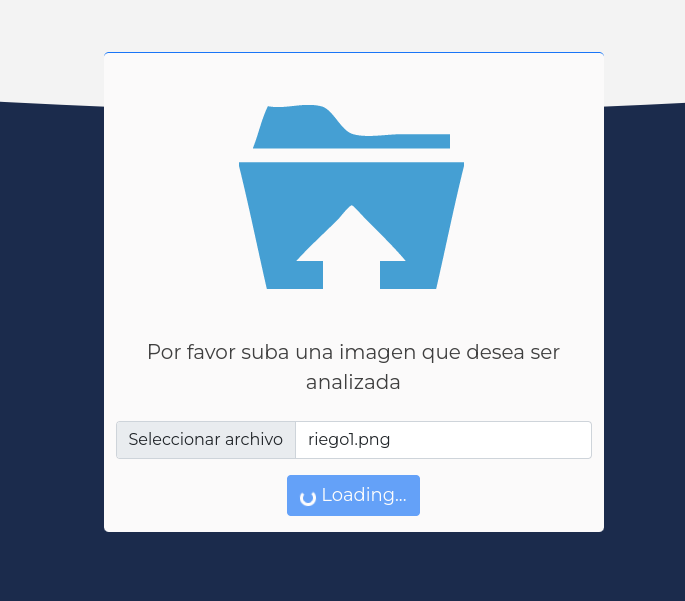
\includegraphics[width=0.6\textwidth]{img/FE - detection loading.png}
    \caption{Inicio de la detección - Loading}
    \label{fig:loading}
\end{figure}

El botón cambiara de nombre y aparece como "Loading", indicando que la detección esta en proceso. Como se puede apreciar en la Figura \ref{fig:loading}.


\subsection{Descarga de imágenes}

Una vez realizada la detección de los objetos, se va a mostrar como resultado las imágenes analizadas indicando la presencia de los objetos Silo bolsas o Riegos por Pívot junto con una tabla donde se detalla la información de la detección.

Luego, se habilitara un botón \textbf{"Download"} que al hacer clic en él, se procede a la descarga de la/s imágenes, como se ve en la Figura \ref{fig:bulk detection} y se debe seleccionar el archivo del destino como se muestra en la Figura \ref{fig:download file}

\begin{figure}[h!]
    \centering
    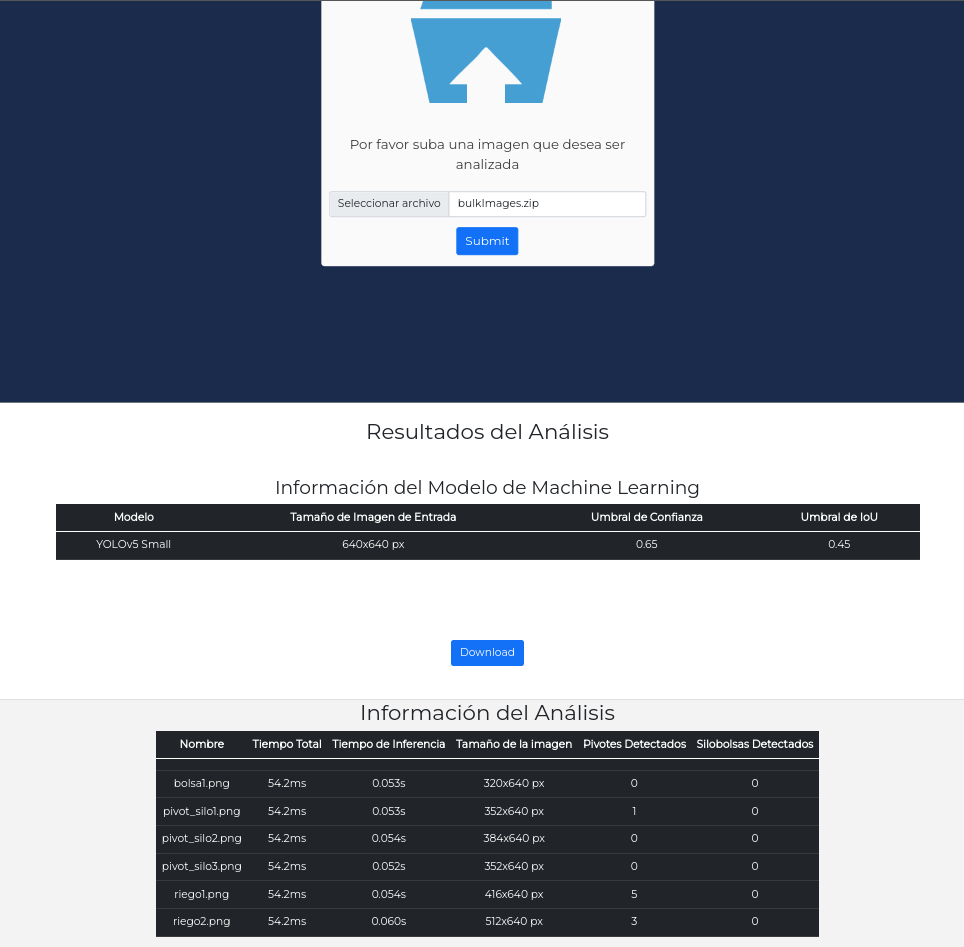
\includegraphics[width=0.93\textwidth]{img/FE - bulk detection.png}
    \caption{Detección de un archivo con imágenes comprimidas}
    \label{fig:bulk detection}
\end{figure}

\begin{figure}[h!]
\centering
    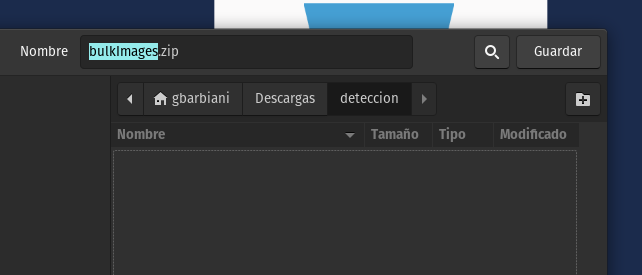
\includegraphics[width=1\textwidth]{img/FE - download file.png}
    \caption{Descarga de archivo con imágenes detectadas - Resultados}
    \label{fig:download file}
\end{figure}

\pagebreak

\subsection{Agradecimientos}

El siguiente proyecto no hubiera sido posible sin el gran trabajo
realizado por Ultralytics que desarrolló el modelo de YOLOv5 en
Pytorch: \url{https://github.com/ultralytics/yolov5}.